\chapter{Introduction}
\label{chapter:introduccion}

\section{Motivation}

The web is filled with billions of images, helping to entertain and inform the world on a countless variety of subjects. However, much of that visual information is not accessible to those with visual impairments, or with slow internet speeds that prohibit the loading of images. Image captions, manually added by website authors using\textit{ Alt-text HTML}, is one way to make this content more accessible, so that a natural-language description for images that can be presented using \textit{text-to-speech} systems. However, existing human-curated \textit{Alt-text HTML} fields are added for only a very small fraction of web images. 
And while automatic image captioning can help solve this problem, accurate image captioning is a challenging task that requires advancing the state of the art of both computer vision and natural language processing.

Automatic image captioning --also called automatic image description--, the task of automatically producing a natural-language description for an image, can help solve this problem when combined with text-to-speech systems.  However, accurate image captioning is a challenging task that requires the joint use of techniques from two research fields: Computer Vision (CV) and Natural Language Processing (NLP).

\begin{figure}
	\centering
	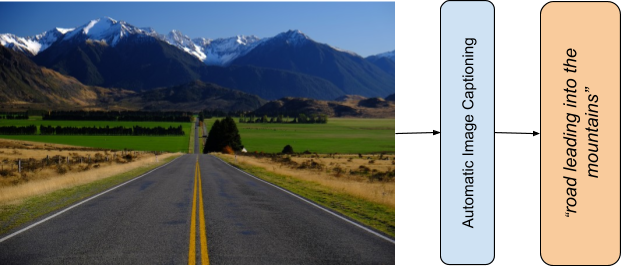
\includegraphics[width=0.6\textwidth]{figs/ch1/image-captioning.png}
	\caption{Image captioning can help millions with visual impairments by converting images captions to text. Image by \href{https://www.flickr.com/photos/francisvallance/}{Francis Vallance (Heritage Warrior)}, used under \href{https://creativecommons.org/licenses/by/2.0/}{CC BY 2.0 license}.}
	\label{fig:image-captioning}
\end{figure}

\section{Goals}

This project aims at advancing in the task of automatically generate image captions. That is the ultimate goal from a very abstract viewpoint. Nevertheless, in order to achieve such an abstract goal, we decompose it into various subgoals, with the aim of achieving at least thee of the them. The subgoals are:

\begin{enumerate}
\item Get a solid understanding of the problem at hand and the state-of-art solutions to it
\item Get practical knowledge on the technologies required to solve this problem
\item Develop a model to be used as a baseline. This model could replicate models that were the state-of-art not so long ago, like the BRNN \cite{Karpathy2017} for the MS-COCO dataset \cite{Lin2014}.
\item Develop a more advanced model using the much larger dataset recently released by Google: the Conceptual Captions Dataset\cite{Sharma2018} (see Figure \ref{fig:conceptual-captions}), and compare with the baseline.
\item Partaking in the \href{https://ai.google.com/research/ConceptualCaptions/}{Conceptual Captions Challenge} introduced recently by Google.
\item Deploy a working prototype for personal, non commercial use by anyone interested. The specific type of product has yet to be defined (could be a telegram bot, a flickr  
\end{enumerate}

\begin{figure}[h]
	\centering
	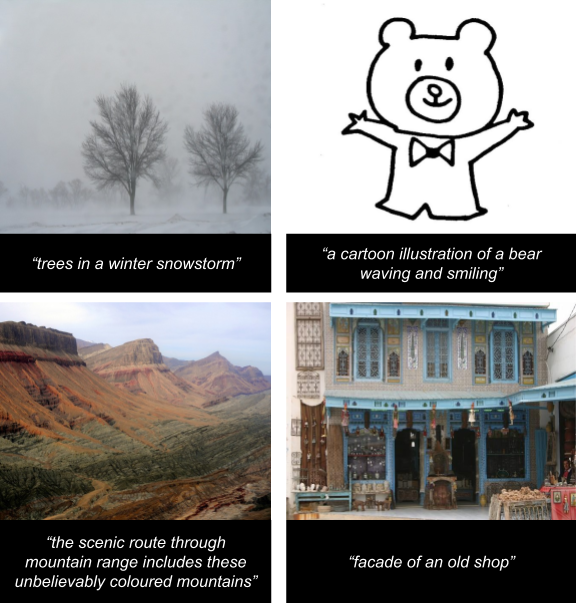
\includegraphics[width=0.6\textwidth]{figs/ch1/conceptual-captions-example.png}
	\caption{Illustration of images and captions in the Conceptual Captions dataset. 
Clockwise from top left, images by Jonny Hunter, SigNote Cloud, Tony Hisgett, ResoluteSupportMedia. All images used under \href{https://creativecommons.org/licenses/by/2.0/}{CC BY 2.0 license}.}
	\label{fig:conceptual-captions}
\end{figure}

\section{Methodology}

This project is mainly an academical, research-oriented project, so it would follow a process model which is common for these kind of projects, for instance, it will include a comparatively long review of the state of the art, as well as a public defense at the end. However, this project will also include the development of a software artifact to solve a data-analytic problem, therefore we should benefit from using a data-analytic model as the well known and widely adopted \textbf{CRISP-DM}. CRISP-DM, which stands for \textit{Cross-Industry Standard Process for Data Mining}, is an open standard process model and an industry-proven methodology to guide data mining projects.

As a methodology, it includes descriptions of the typical phases of a project, the tasks involved with each phase, and an explanation of the relationships between these tasks.

As a process model, CRISP-DM provides an overview of the data mining life cycle.

Figure \ref{fig:crisp-dm} depicts the relationships between the different phases of the CRISP-DM model. The sequence of the phases is not strict and moving back and forth between different phases is often required. The arrows in the process diagram indicate the most important and frequent dependencies between phases. The outer circle in the diagram symbolizes the cyclic nature of data mining itself. A data mining process continues after a solution has been deployed. The lessons learned during the process can trigger new, often more focused business questions, and subsequent data mining processes will benefit from the experiences of previous ones.

\begin{figure}[hpt]
	\centering
	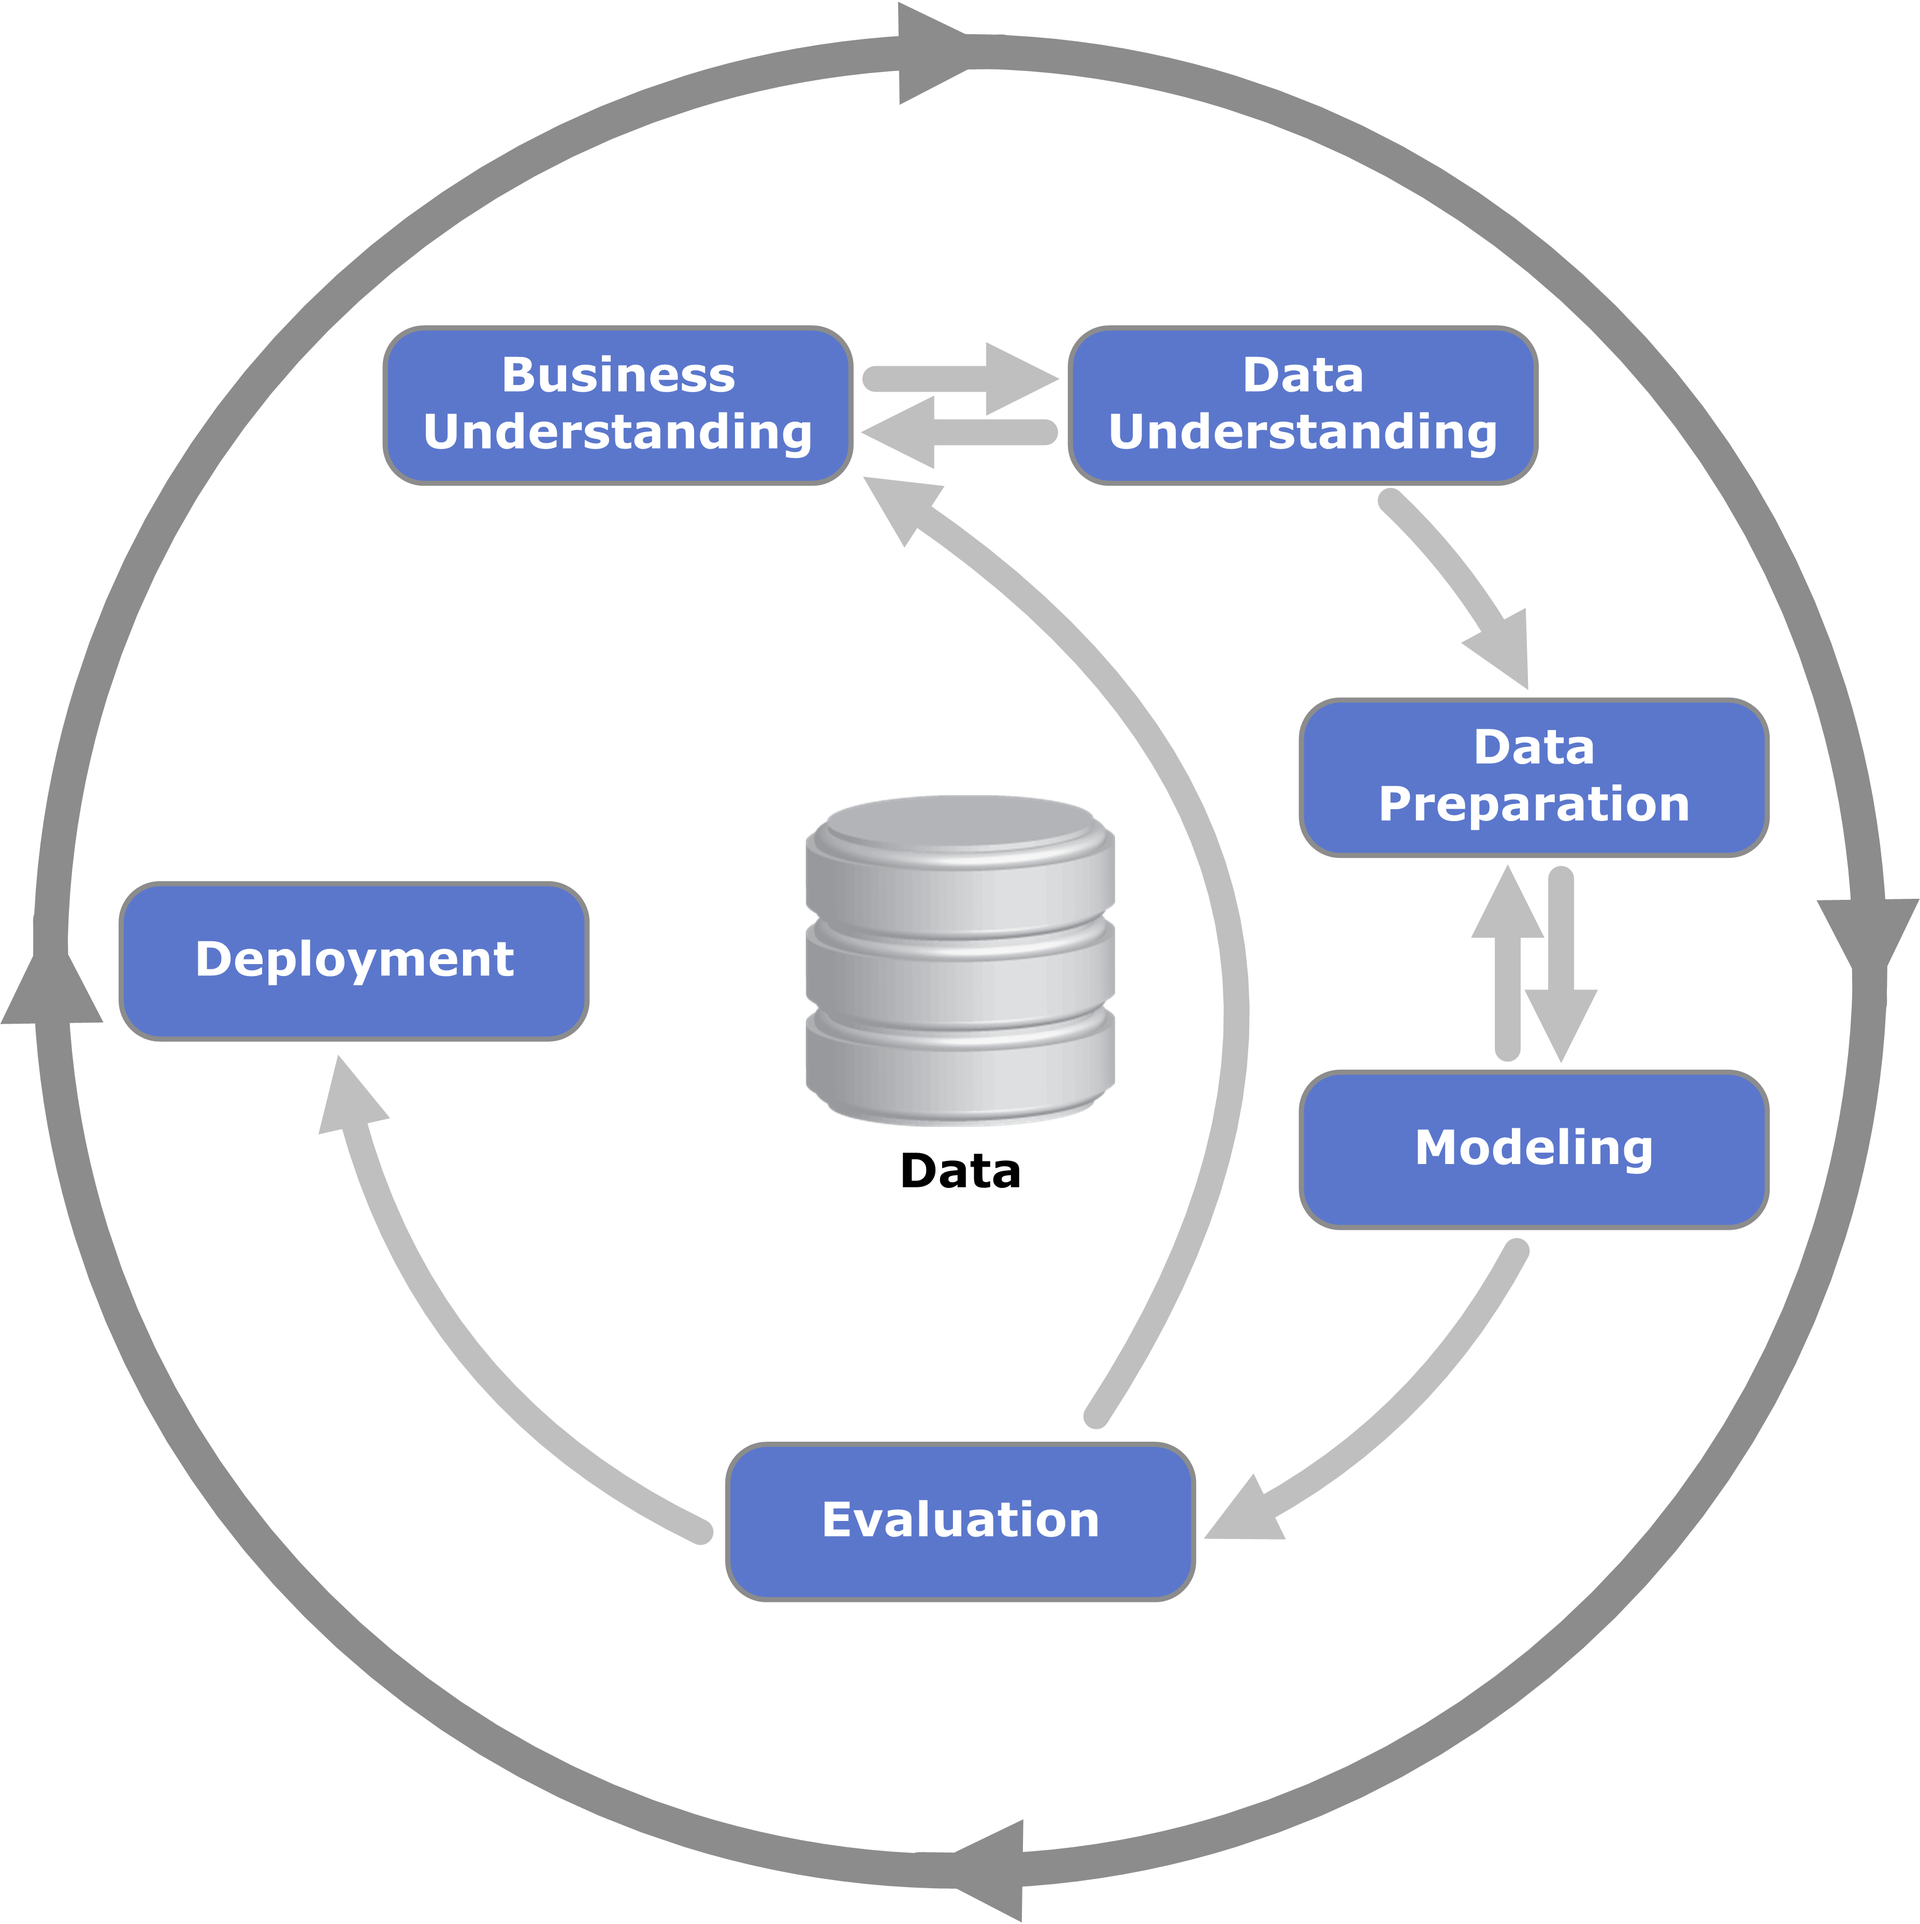
\includegraphics[width=0.6\textwidth]{figs/ch1/crisp-dm.png}
	\caption{Process diagram showing the relationship between the different phases of CRISP-DM. Image by Kenneth Jensen, used under \href{https://creativecommons.org/licenses/by/2.0/}{CC BY-SA 3.0 license..}}
	\label{fig:crisp-dm}
\end{figure}

The process model consists of six major phases:

\begin{itemize}
\item \textbf{Business Understanding}: Includes an in-depth analysis of the business objectives and needs. The situation is assessed and the goals of the project are defined. This should follow the setting up of a plan to proceed.
\item \textbf{Data Understanding}: Conduct initial or exploratory data analysis to become familiar with data and identify potential problems. Examine properties of data and verify its quality by answering questions concerning the completeness and accuracy of the data.
\item \textbf{Data Preparation}: After the data sources are completely identified, proper selection, cleansing, constructing and formatting should be done before modelling. 
\item \textbf{Modeling}: Modeling is usually conducted in multiple iterations, which involve running  several models using the default parameters and then fine-tune the parameters or revert to the data preparation phase for additional preparation. Usually, there are different ways to look at a given problem, so it is convenient to build multiple models,
\item \textbf{Evaluation}: The results of models are evaluated in the backdrop of business intentions. New objectives may sprout up owing to the new patterns discovered. This is, in fact, an iterative process, and the decision whether to consider them or not has to be made in this step before moving on to the final phase
\item \textbf{Publication}. The final information gathered has to be presented in a usable manner to the stakeholders.  This has to be done as per their expectations and business requirements.
\end{itemize}


\section{Planning}

Main tasks and milestones

\begin{table}[hbt]
\begin{tabular}{|l|l|l|}
\hline
Phase   & End  & Description   \\ \hline
1 & 3/3/2019 & Definition and planning  \\ \hline
2 & 24/3/2019 & State of the Art \\ \hline
3 & 19/5/2019 & Development \\ \hline
4 & 9/6/2019 & Complete this report \\ \hline
5 & 16/6/2019 & Presentation
\end{tabular}
\end{table}

Phase 2: this phase will encompass the following tasks:
\begin{itemize}
\item Reviewing relevant bibliography
\item Studying the problem domain (business understanding), and becoming familiar with the data. At this stage we would also start preparing the data for the modeling stage
\end{itemize}

Phase 3: this will be the longest phase, and it will include the following tasks  
\begin{itemize}
\item Preparing the data. Although data preparation could be started during phase 2, depending on the chosen models it could be necessary to conduct some additional data preparation operations
\item Generating one or various models. We plan at creating at least two models, one that would replicate existing work, and another one to explore new ideas and try to beat the baseline model.
\item Evaluating the models, and very specifically, compare our model against the replicated model.
\item Publication: We consider two courses of action: a) participating in the Conceptual Captions Challenge by Google, and b) delivering some product to the final user, although it would be a very basic prototype given the little time available.
\end{itemize}

In phase 4 we will complete this report. We would probably overlap this task with some of the tasks in phase 3 that will required more time, like the evaluation of the models and the participation in challenges.

In phase 5 we will present the results achieved for its evaluation. These results will include the code, the documentation and a public defense of the project in front of an academic board

